\FloatBarrier
\section{Aufgabe 3}
\label{sec:A3}
\subsection*{a)}
\begin{figure}
\centering
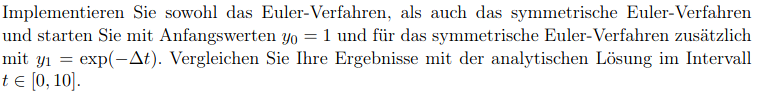
\includegraphics[width=\textwidth]{bild/a.png}
\end{figure}
\begin{figure}
    \centering
    \includegraphics[width=\textwidth]{code/build/a3_a.pdf}
\end{figure}
\begin{figure}
    \centering
    \includegraphics[width=\textwidth]{code/build/a3_a_diff.pdf}
\end{figure}
\FloatBarrier
In der Abbildung mit den Differenzen zu den analytischen Werten
kann man erkennen, dass bei dem Eulerverfahren, 
die Differenz kleiner wird je mehr Punkte berechnet werden.
Bei dem symmetrischen Eulerverfahren nicht die Differenz zu und osziliert
von negativen zu positiven Abweichungen.
\FloatBarrier
\subsection*{b)}
\begin{figure}
\centering
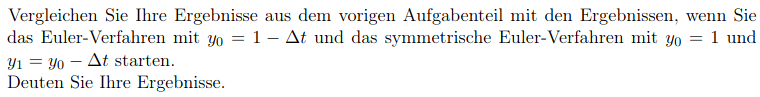
\includegraphics[width=\textwidth]{bild/b.png}
\end{figure}
\begin{figure}
    \centering
    \includegraphics[width=\textwidth]{code/build/a3_b.pdf}
\end{figure}
\begin{figure}
    \centering
    \includegraphics[width=\textwidth]{code/build/a3_b_diff.pdf}
\end{figure}
\FloatBarrier
Vergleicht man die Abweichung mit Teil a) sind diese größer.
Das heißt wie gut das Verfahren für das Problem ist, ist abhängig von den Startbedingungen.
